\documentclass{article}
\usepackage[utf8]{inputenc}
\usepackage{graphicx}
\usepackage{biblatex}
\addbibresource{gradProjBib.bib}
\begin{document}

\title{Text Classification using Markov Model Transition Probabilities}
\author{Anna Marbut}
\date{Machine Learning Grad Project - Fall 2020}


\maketitle

\section{Introduction}
Classification of text data is a major area of study in Computational Linguistics both due to its utility and its difficulty. While it's nearly impossible to measure how well a computer model ``understands" written language, using a model to place documents into categories gives us some insight into how well the model matches human interpretation. There are many common methods that require the algorithm to discover these categories based on the data itself (called unsupervised learning), however interpretation of the classification results is much easier if the categories are predetermined (called supervised learning). On the other hand, supervised methods require that labeled training data be available, which limits the number of datasets that can be used to explore these methods.

Many natural language processing (NLP) classification methods treat documents as collections of words, regardless of word order--often referred to as bag-of-words models \cite{tidytext}. These methods will compare word frequency based measures between documents and between classes in order to determine probability of class-membership. In addition to losing semantic information that might be expressed by word order (such as negation or modifiers such as adjectives and adverbs), these bag-of-words methods are often computationally expensive. Each document is represented as a vector of word counts for all words in the corpus (collection of documents), which creates a vector space model (VSM) for the corpus with dimensions $n =\ the\ total\ number\ of\ distinct\ words\ in\ all\ documents\ $ by $m =\ the\ total\ number\ of\ documents\ $ \cite{bagOfWords}. This $n \times m$ representation becomes impractical quickly as the number of distinct words and documents in the dataset increases.

Using a Markov Model for text classification is one method that addresses both the word-order/context and space requirement issues that arise with VSMs. For classification tasks, Markov Models can be used to create transition matrices for each class, such that the probability of seeing a word given the preceding word will differ between classes. These transition matrices can then be applied to documents in the testing set to produce a probability of class membership given the string of words in each document \cite{textMining}. Al-Anzi and AbuZeina \cite{arabic} use a Markov Model for hierarchichal classification of Arabic text and show only minor losses in classification accuracy with major improvements in the space-requirements compared to VSMs applied to the same task. Hoffmeister and Zeugmann \cite{textMining} apply Markov Chains of different lengths (computing the probability of seeing a word given the preceding n words) to classification tasks on the Reuters data set and find some improvement over methods that don't consider word-order/context. Yi and Beheshti \cite{hmmMed} also show comparable accuracy to VSMs with a more scalable implementation using a hidden markov model to classify medical documents.


\section{Data Description}
The corpus of documents used in this paper consists of the titles and guidelines texts for a collection of online forms from the Submittable software platform. The labels applied to each document are meant to reflect the purpose for which an organization is using the software and are applied by a sales representative at the time the software is purchased or renewed. These labels, referred to as use cases and listed in Table \ref{tab:ucCounts}, are not well-defined and each organization may be labelled with any number of them. Additionally, an organization may end up using the software for purposes other than the one they initially imagined, which would not be reflected in the use case labels applied to them.

\begin{table}[h]
    \centering
    \begin{tabular}{c|c|c}
    \hline
         Use Case & Number Training Forms & Use Case Group \\
    \hline
         Admissions & 114 & Group 2 \\
         Audition & 203 & Group 2 \\
         Award/Nomination & 446 & Group 1 \\
         Conference & 107 & Group 3\\
         Contest & 585 & Group 3\\
         Exhibition & 227 & Group 3\\
         Fellowship & 236 & Group 1\\
         Festival or Event & 131 & Group 3\\
         Grants & 1074 & Grants\\
         Internal Use & 27 & Group 2\\
         Internships & 6 & Group 1\\
         Job applications & 24 & Group 2\\
         Publishing & 2147 & Publishing\\
         Residency & 136 & Group 1\\
         Scholarships & 210 & Group 1\\
    \end{tabular}
    \caption{Use case labels and their distribution among the training data set}
    \label{tab:ucCounts}
\end{table}

The goal of this paper is to predict a single use case for a form given its title and guidelines text. To this end, the training data was limited to relatively new (created since 2018) organizations with only one listed use case, with the assumption that the forms for these organizations would fall under that single use case with some reliability. This resulted in a training set of 5673 forms, with the distribution among the use cases seen in Table \ref{tab:ucCounts}. Given this uneven distribution of the training data as well as the semantic overlap between many of the use cases, a second grouping was created to even out the distribution and merge similar labels (column 3 in Table \ref{tab:ucCounts}).

With the already limited number of labelled forms available using the filtering process described above, two testing sets were manually labelled for the two sets of use cases. The first testing set consisted of 10 forms for each of the 15 use cases in column 1 of Table \ref{tab:ucCounts}. The second testing set consisted of 50 forms for each of the 5 use case groups in column 3 of Table \ref{tab:ucCounts}. Although this method of testing set creation is not ideal and may reflect bias in the manual labelling and selection process, it allowed all 5673 forms selected above to remain in the training set and ensured that the use case labels in the testing set were accurate and reliable.


\section{Methods}
\subsection{Pre-Processing}
In order to avoid creating two or more entries for words based on different capitalization, the text in both form names and form guidelines was all converted to lower case. In addition to this step, html formatting was removed from the form guidelines text using the python lxml library. This removed any formatting marks and functions that would not have been visible in a browser, including raw urls. Finally, the text was split into individual words and punctuation based on whitespace, without any changes to word/punctuation order.

\subsection{Modeling}
Generally, Markov Models rely on the assumption that the probability of seeing any given outcome relies on a fixed number of preceding outcomes \cite{textMining}. In this paper, we explore a first order Markov Model in which the probability of seeing any specific word, $W_{t+1}$, relies only on the immediately preceding word, $W_{t}$, such that $$P(W_{t+1})=P(W_{t+1}|W_{t})P(W_{t})$$ where each of these probabilities are computed naively from the training set. $$P(W_{t})=\frac{\#\ of\ times\ W_{t}\ occurs}{Total\ \#\ of\ words}$$ $$P(W_{t+1}|W_{t}) = \frac{\# \ of\ times\ W_{t+1}\ follows\ W_{t}}{\# \ of\ times\ W_{t}\ occurs}$$ Thus, each word in the training data can be represented as a vector of transition probabilities to following words, all of which sum to 1. We computed separate transition probability vectors for each use case in both of the two use case schemata based on form name alone and form guidelines alone.

\subsection{Testing}
We then applied these transition probability vectors to each form in the testing data to compute the log-likelihood of class membership for each use case. In order to account for words and transitions that were not seen in the training data, an unknown probability of $p=10^{-9}$ was applied to unseen words and a regularization factor of $\lambda = 0.01$ was included in the log-likelihood equation $$\texterm{log\ likelihood}\ = \sum_{t=1}^{n} log((1-\lambda)\times P(W_{t+1}|W_{t}))+(\lambda \times P(W_{t}))$$ Finally, the use case with the highest log-likelihood was selected as the model's prediction for class membership and compared to the manually applied use case label to measure the model's accuracy.

\section{Results}

As seen in Figures \ref{fig:nameConfusion} and \ref{fig:descConfusion}, the models based on all 15 original use cases do a poor job of predicting the correct use case with 16.7\% and 16\% accuracy based on form name and form guidelines, respectively. 
\begin{figure}[h!]
    \centering
    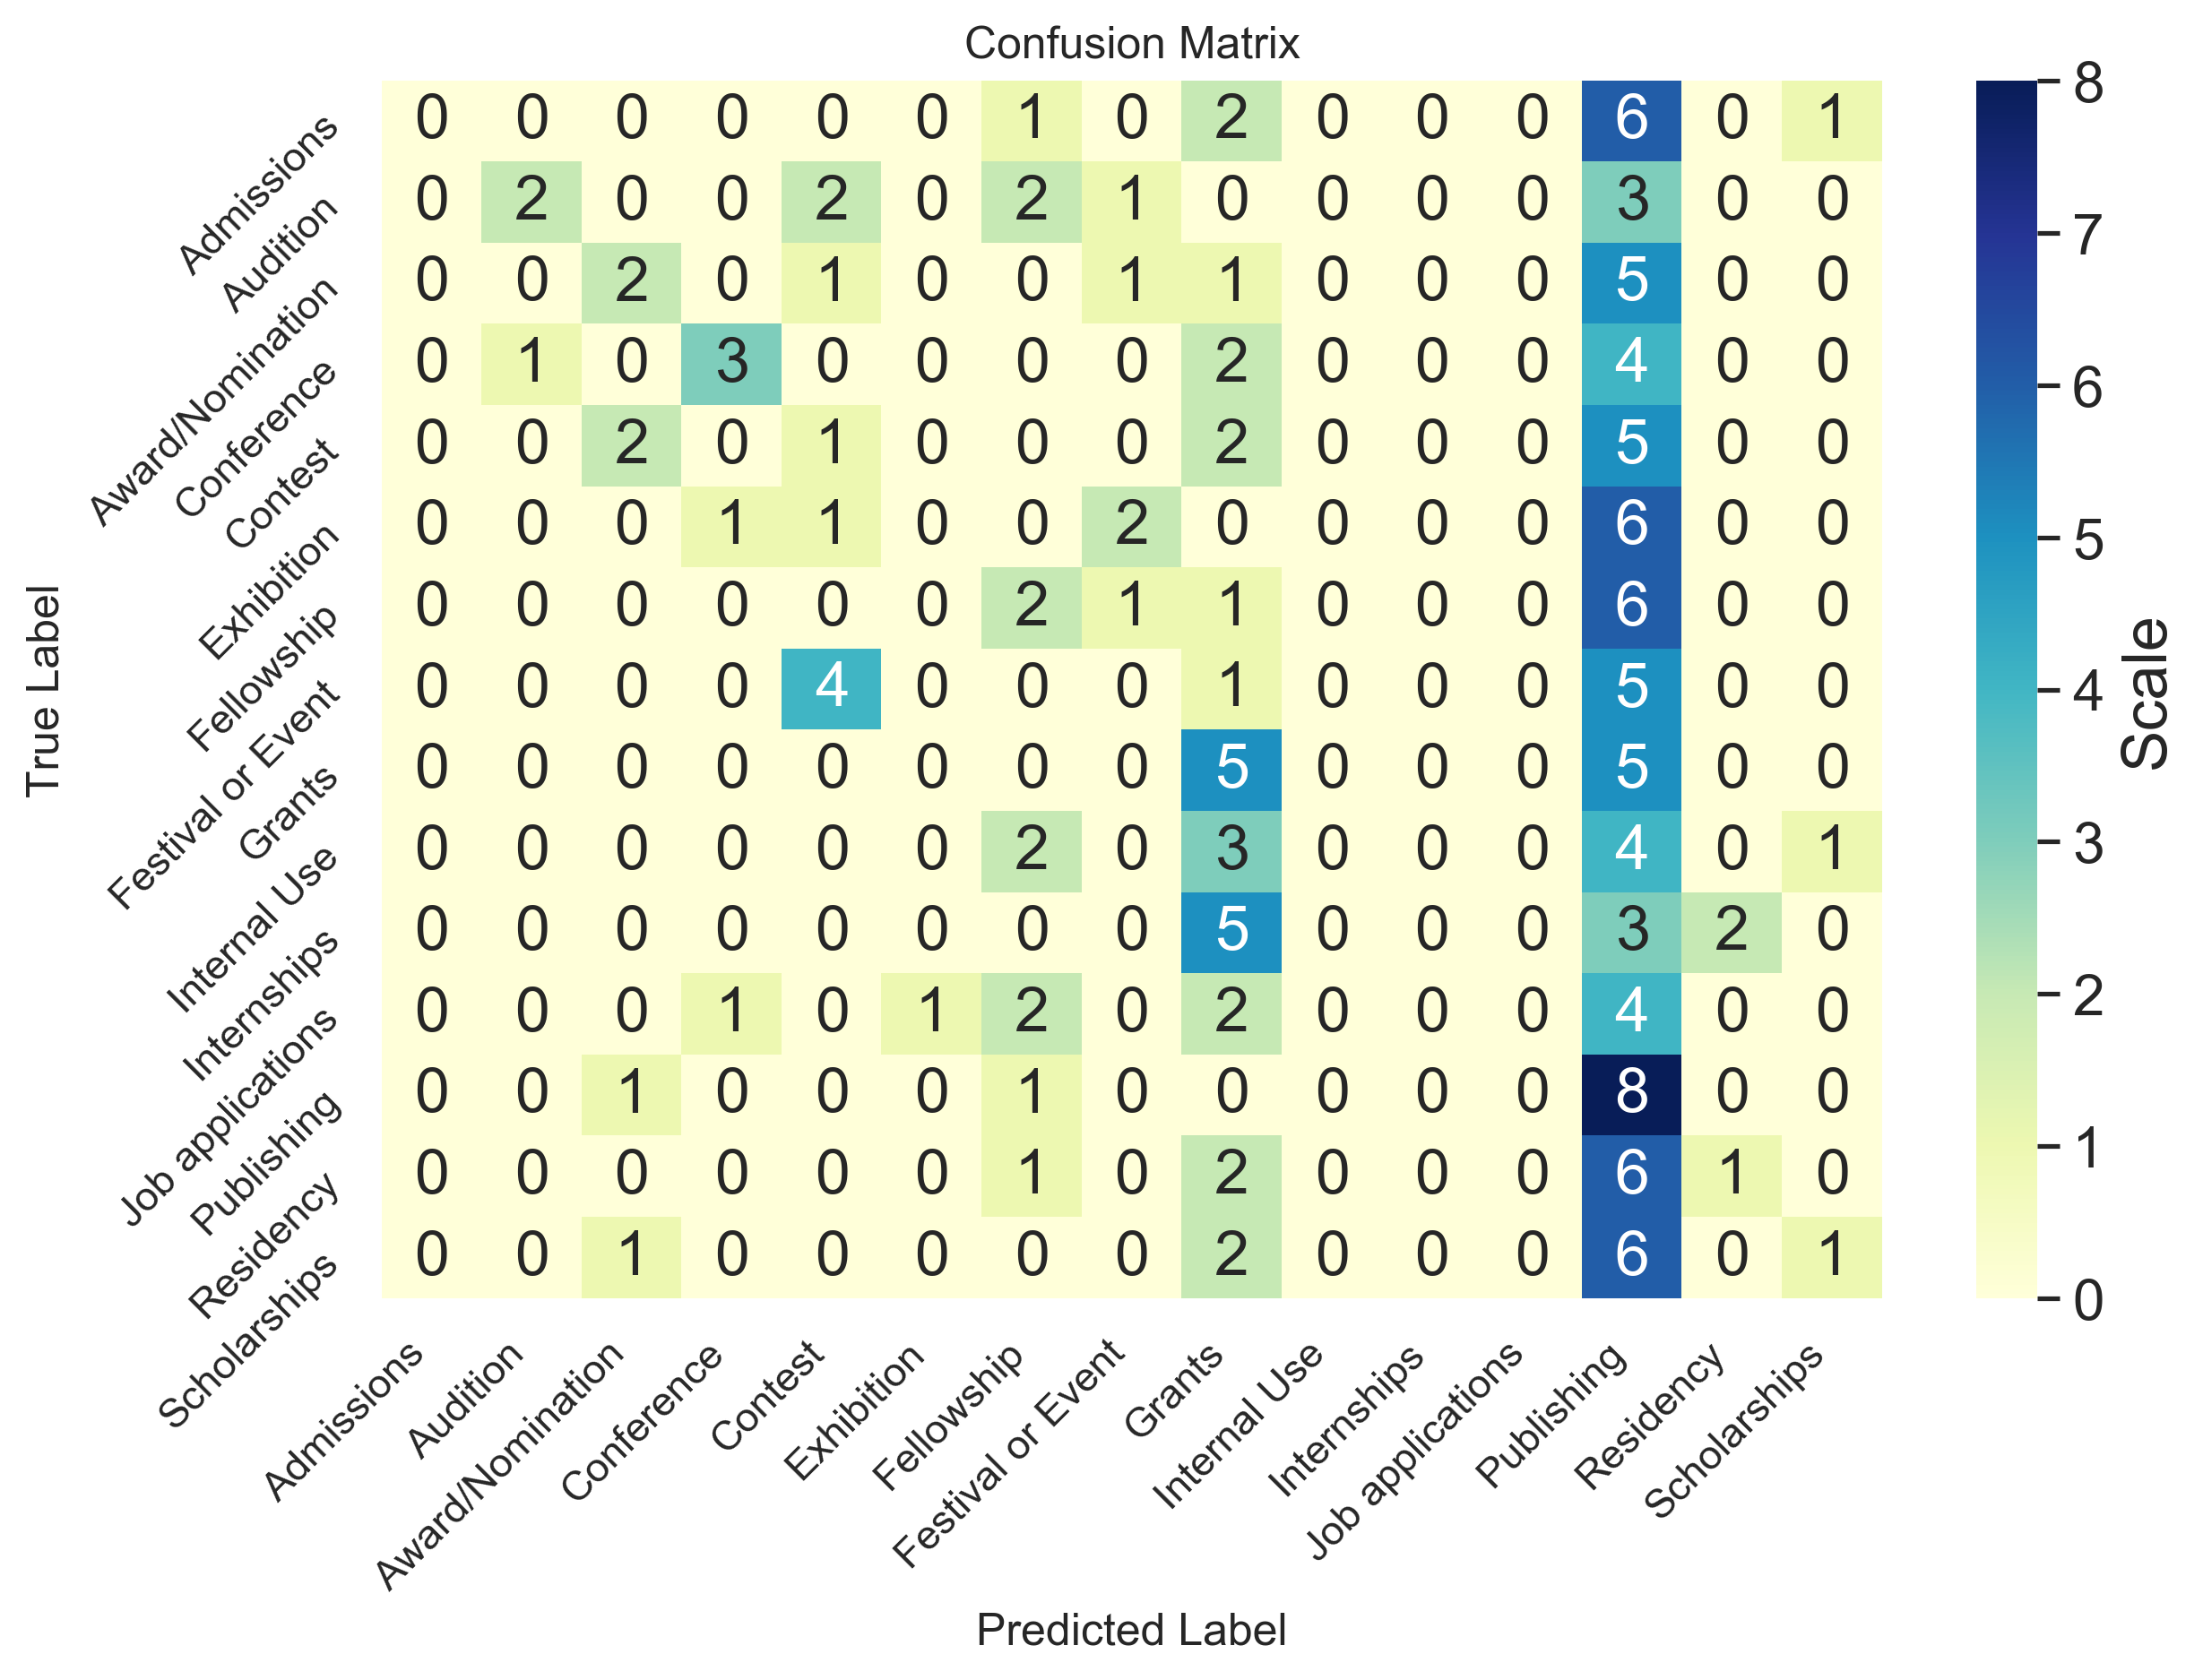
\includegraphics[width=0.8\textwidth]{nameConfusion.png}
    \caption{Confusion matrix of form classification based on form name. There are 10 forms for each use case in the testing set.}
    \label{fig:nameConfusion}
\end{figure}

\begin{figure}[h!]
    \centering
    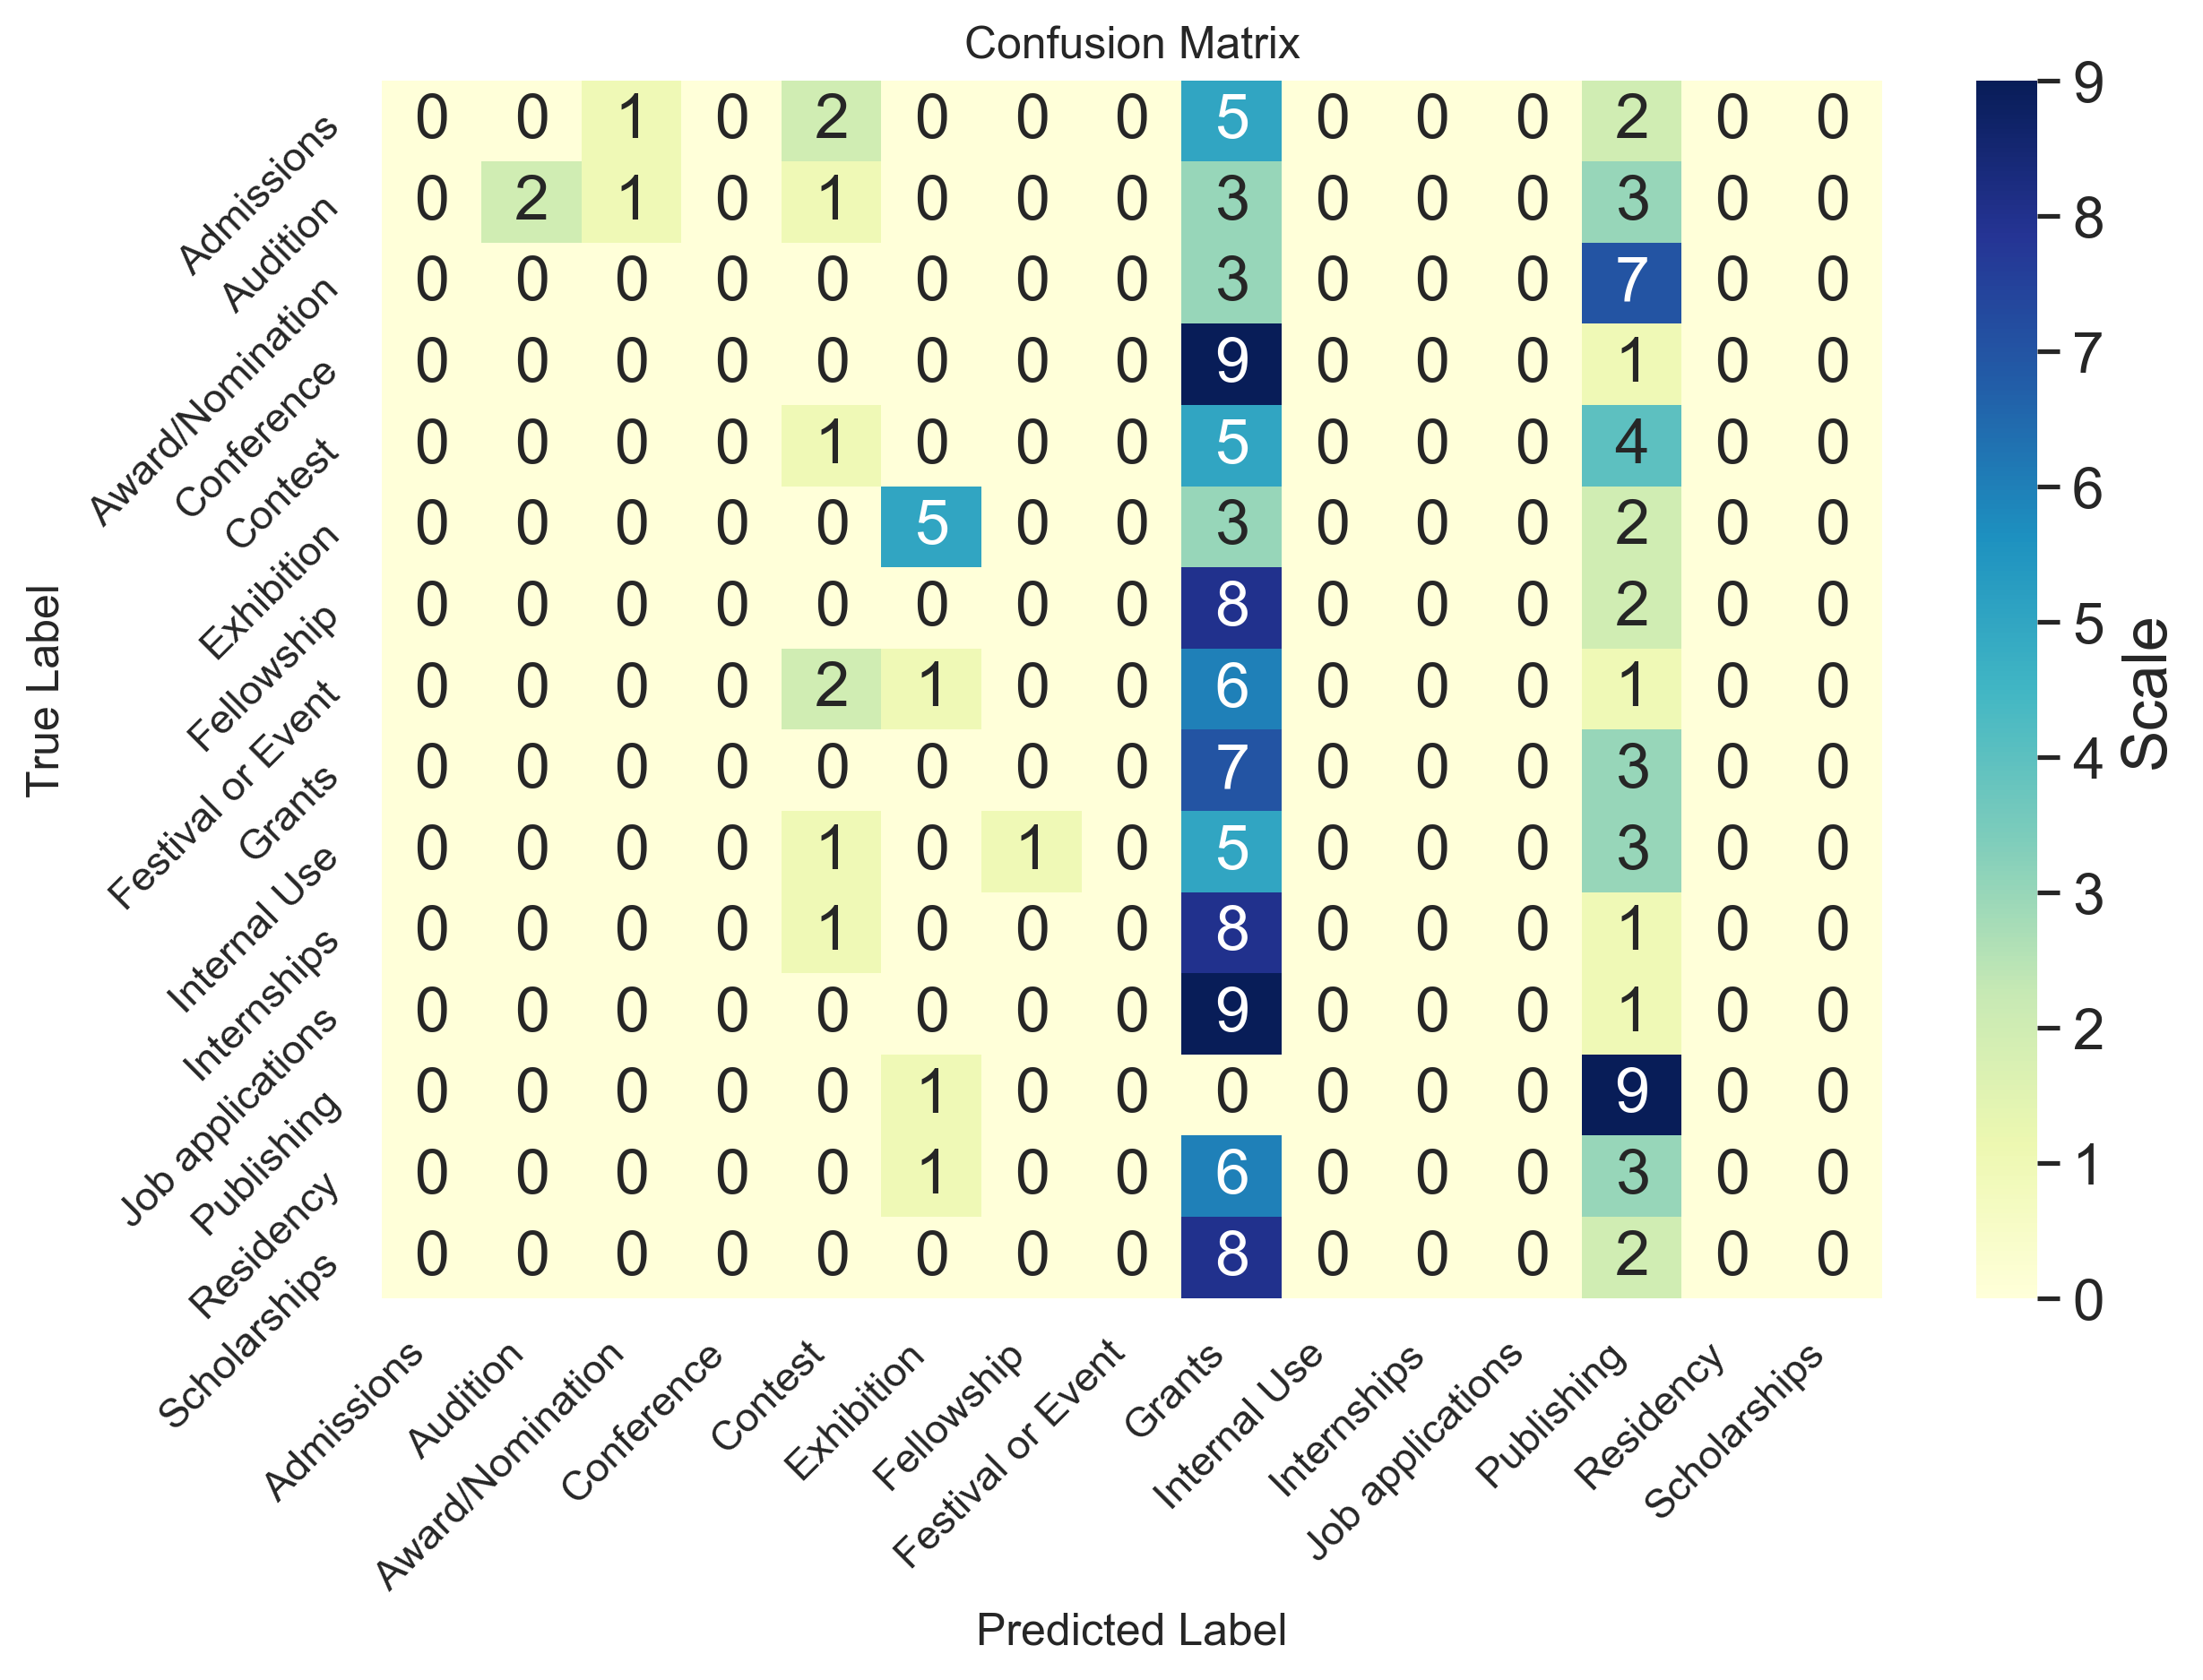
\includegraphics[width=0.8\textwidth]{descConfusion.png}
    \caption{Confusion matrix of form classification based on form guidelines. There are 10 forms for each use case in the testing set.}
    \label{fig:descConfusion}
\end{figure}


Using the grouped use cases, we see some improvement in the models' predictions in Figures \ref{fig:newNameConfusion} and \ref{fig:newDescConfusion}. With these grouped models, we saw 37.6\% and 48.4\% accuracy based on form name and form guidelines, respectively.

\begin{figure}[h!]
    \centering
    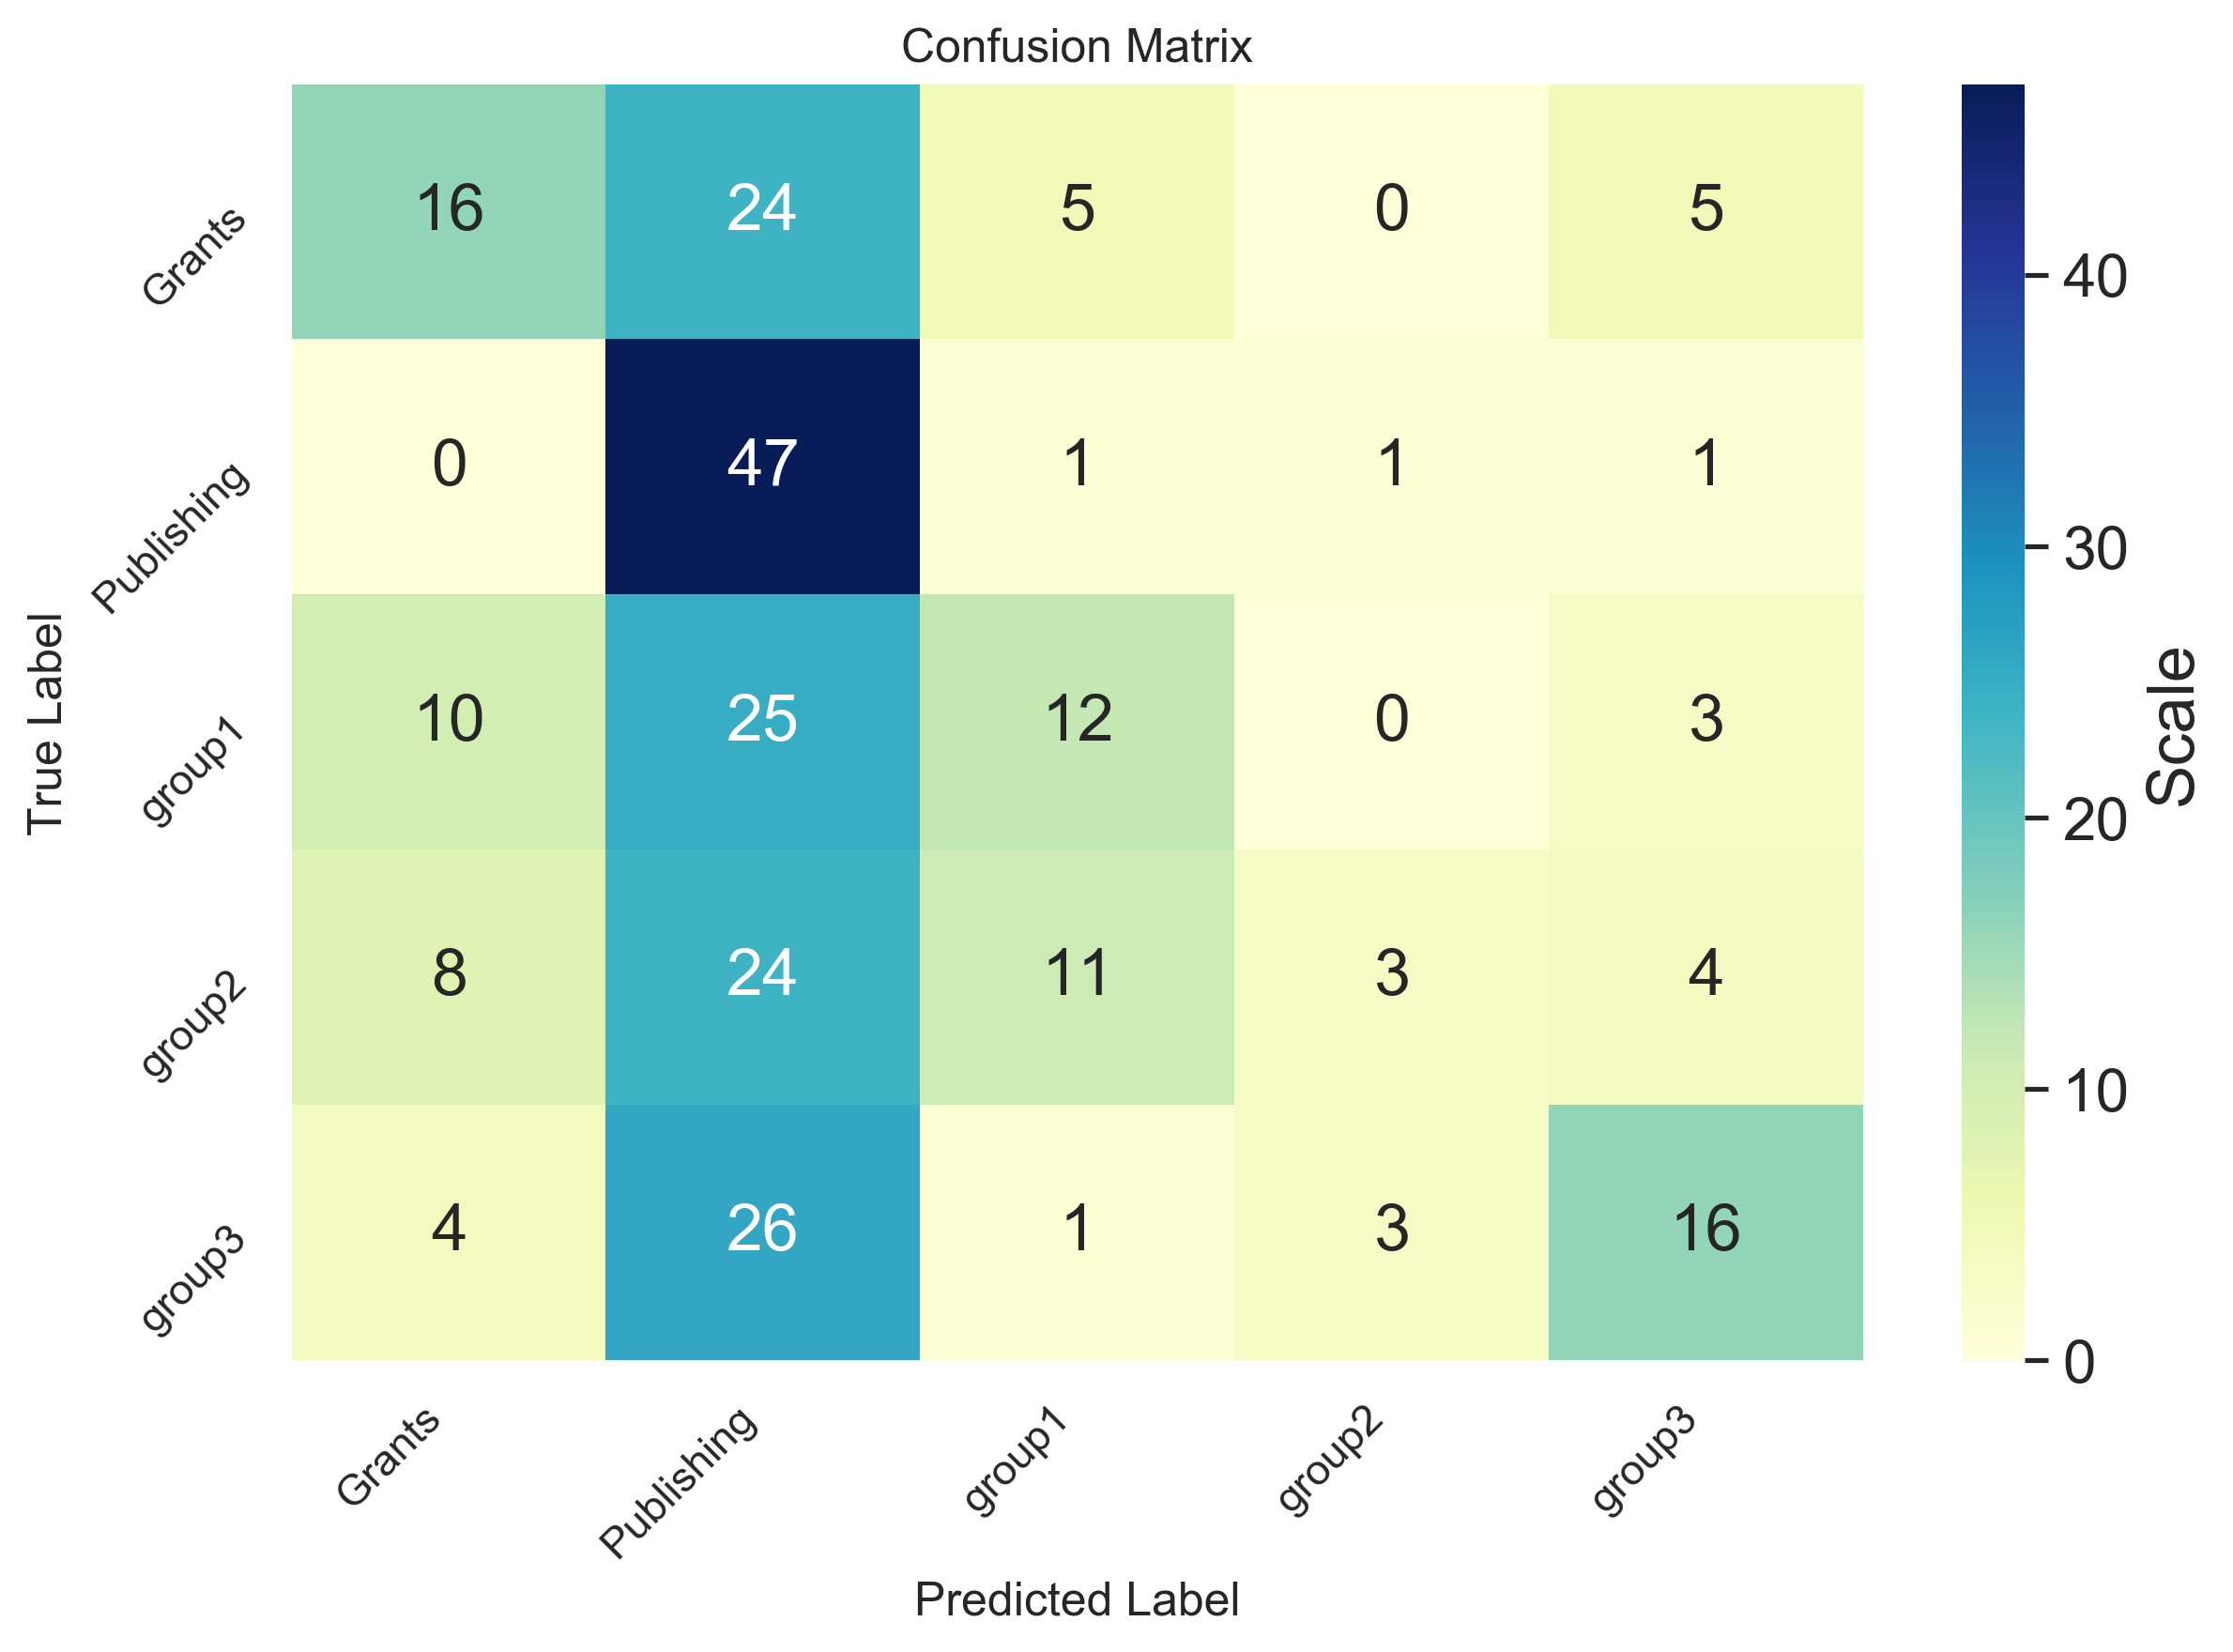
\includegraphics[width=.8\textwidth]{newNameConfusion.png}
    \caption{Confusion matrix of form classification based on form name with grouped classes. There are 50 forms for each use case group in the testing set.}
    \label{fig:newNameConfusion}
\end{figure}

\begin{figure}[h!]
    \centering
    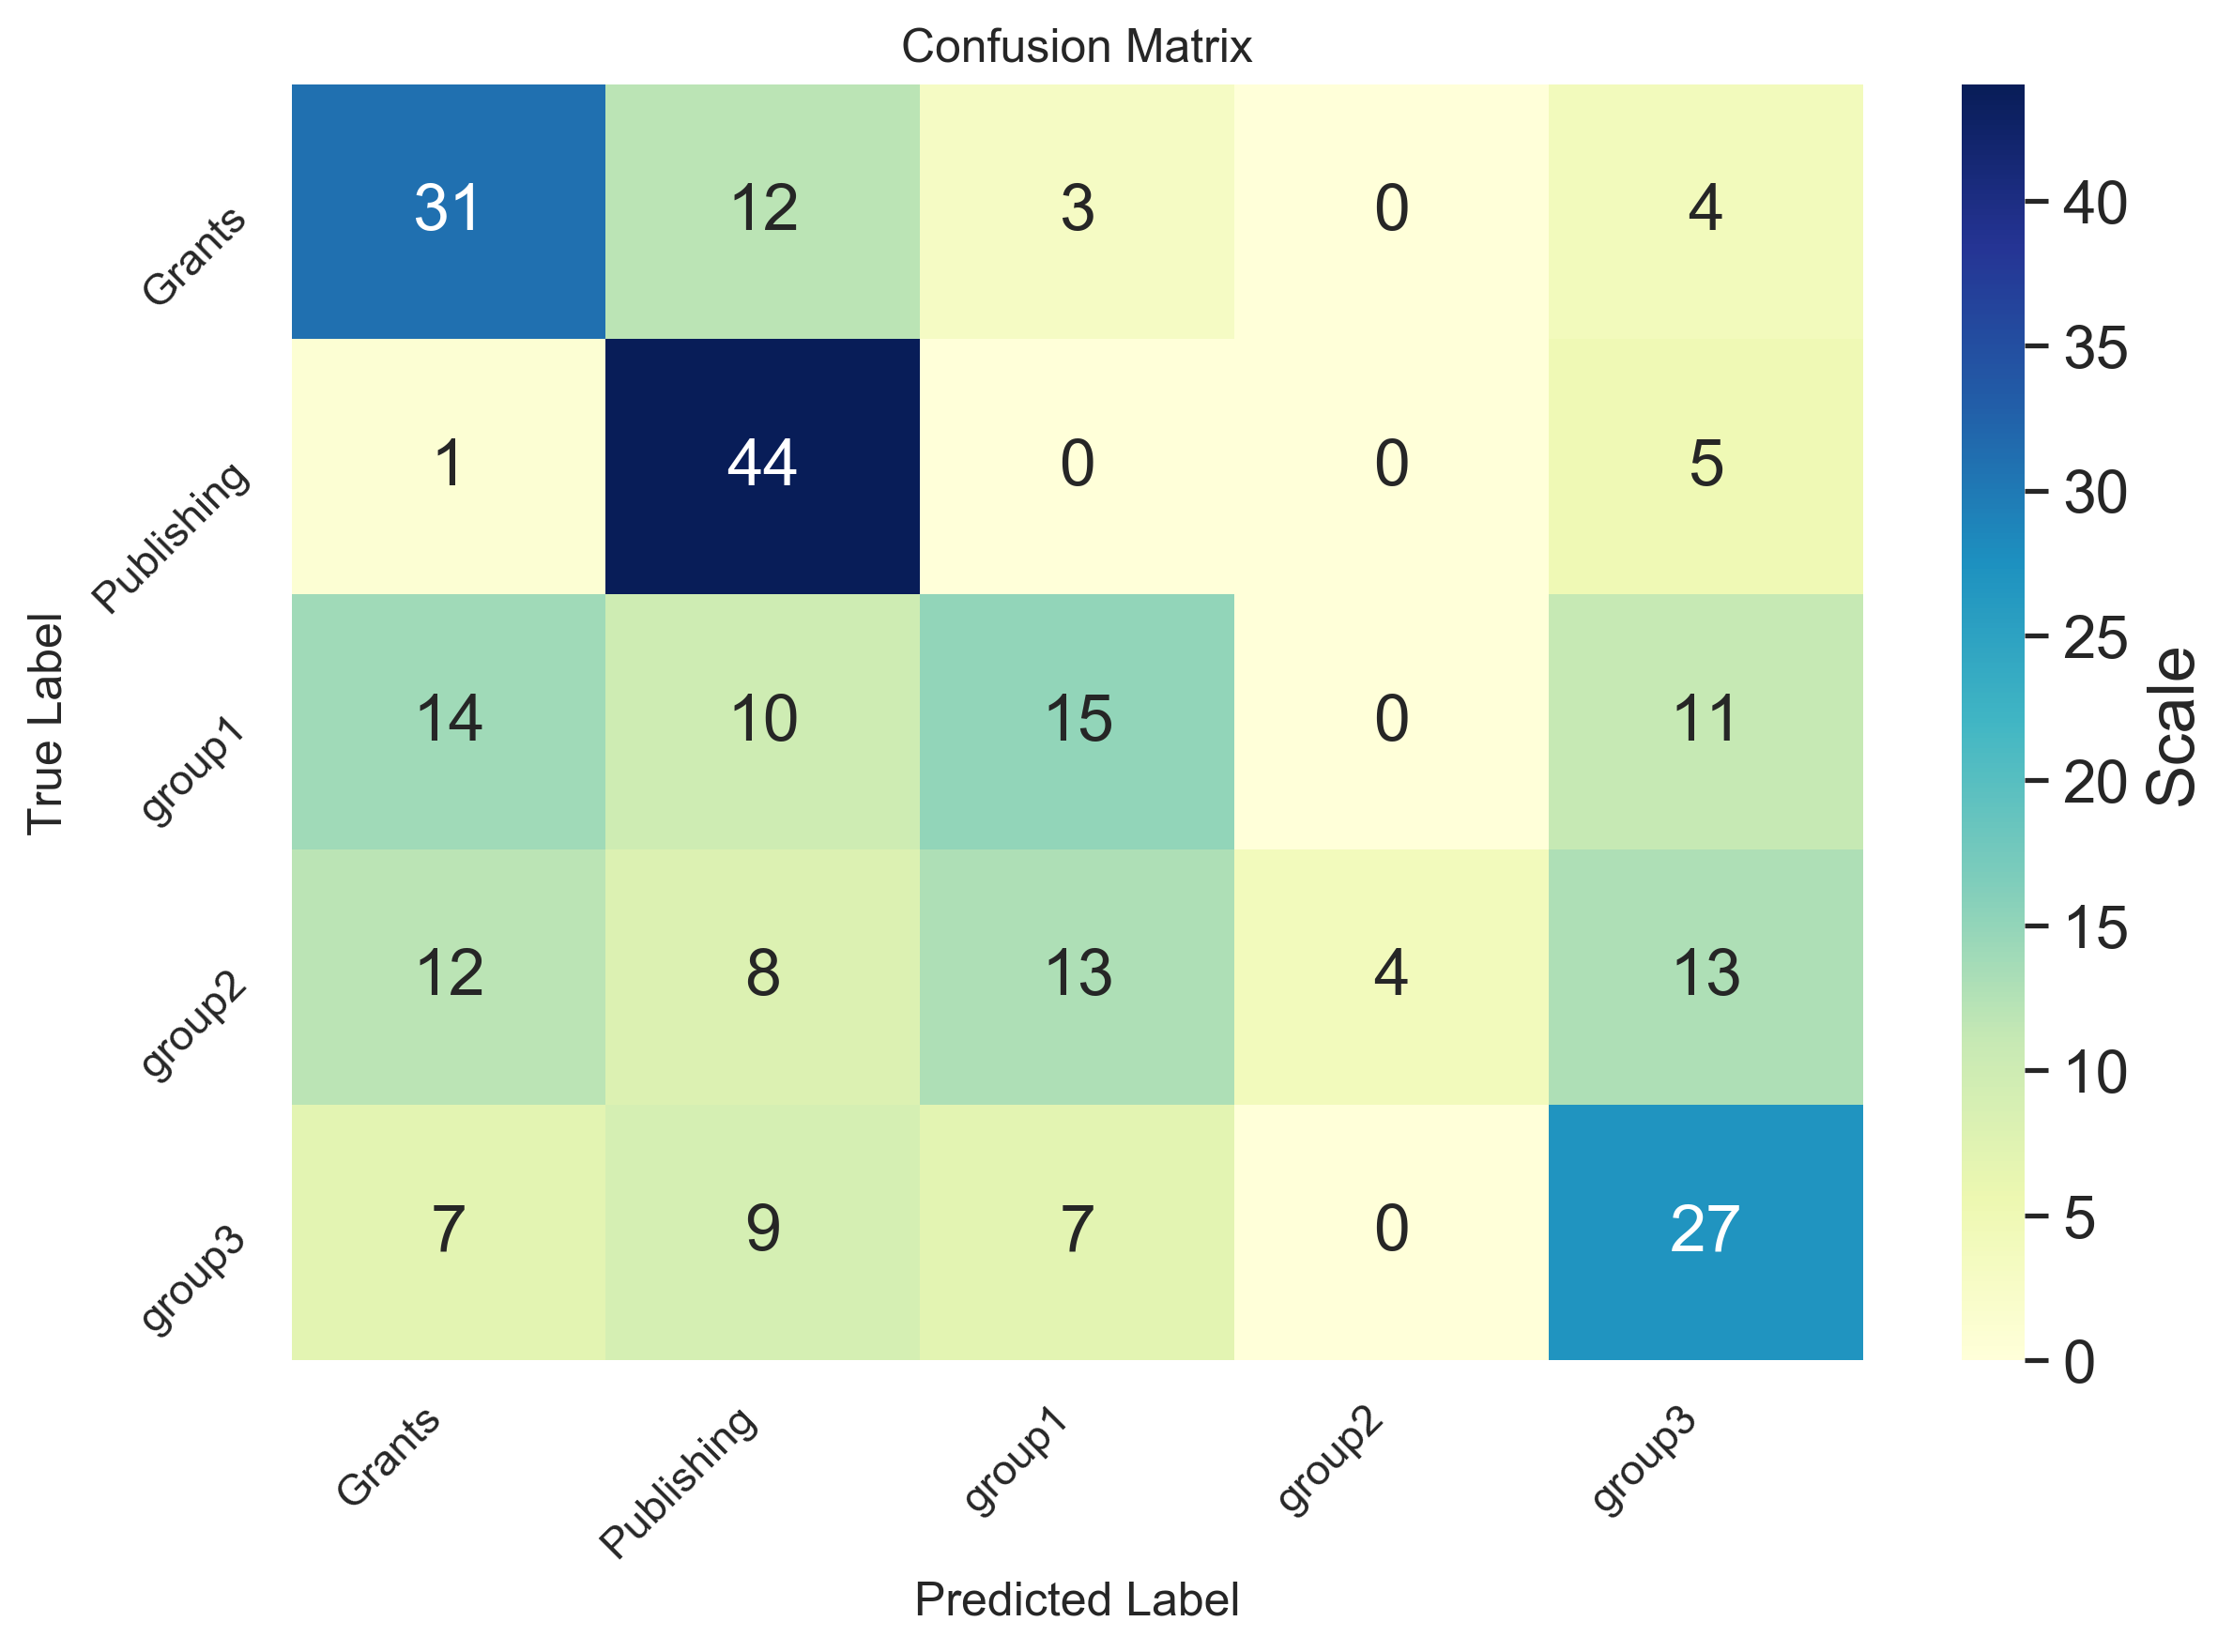
\includegraphics[width=.8\textwidth]{newDescConfusion.png}
    \caption{Confusion matrix of form classification based on form guidelines with grouped classes. There are 50 forms for each use case group in the testing set.}
    \label{fig:newDescConfusion}
\end{figure}

\section{Discussion}
The effect of the uneven distribution in the training data is especially apparent in Figures \ref{fig:nameConfusion} and \ref{fig:descConfusion}, where almost all of the use case predictions fell into the two categories with the majority of the training data, Grants and Publishing. Logically, this makes sense since these two classes would have had more variation in the text used in training just by virtue of having more words. This results in non-zero transition probabilities for a larger number of words, such that the unknown probability value, which we expect to be much smaller than the calculated transition probabilities, would not need to be used as often in these two use cases as in the others. With fewer of these almost-zero transition probabilities, the log-likelihood for these two classes will be higher than those for the other use cases, even if they're still not very high.

This effect is still present in the grouped use case models, although to a lesser degree since the distribution of training data between the use case groups was less varied. Still, Group 2 (Job applications, Internal Use, Admissions, and Audition) had only 368 forms in the training data, compared to over 1000 for each of the other four classes, and we see that Group 2 also had the fewest predicted labels.

Although the performance of these models is nowhere near where we'd like to see it, it's worth noting that it's still better than chance, in which we'd expect to see correct predictions in 6.7\% of forms when using all 15 use cases, or in 20\% of forms when using the grouped use cases. Given the known issues with the use cases we were trying to predict, these results are encouraging for the effectiveness of the methodology more generally. We plan to perform more work on this data set, addressing the issue of overlapping classes and creating a reliable training set that's more evenly distributed among a new list of use cases. Once this higher quality data is available, we will re-apply the methodology seen in this paper, as well as other supervised classification techniques.

\printbibliography

\end{document}
